In this section will be presented an overview of the user’s interface of the CKB platform.
The focus will be mainly on the user experience. 
\verb|CKB| is accessible using any browser and does not havea client application.
Images shown below depicting the user interface include both samples for the desktop browser version and the mobile version.

\section{General Overview}
\label{sec: general_overview}%
The image below shows a map of the pages which can be accessed from the web application.
All pages are available after the user has logged in, except for the registration page and the login page itself.

\begin{figure} [H]
    \begin{center}
        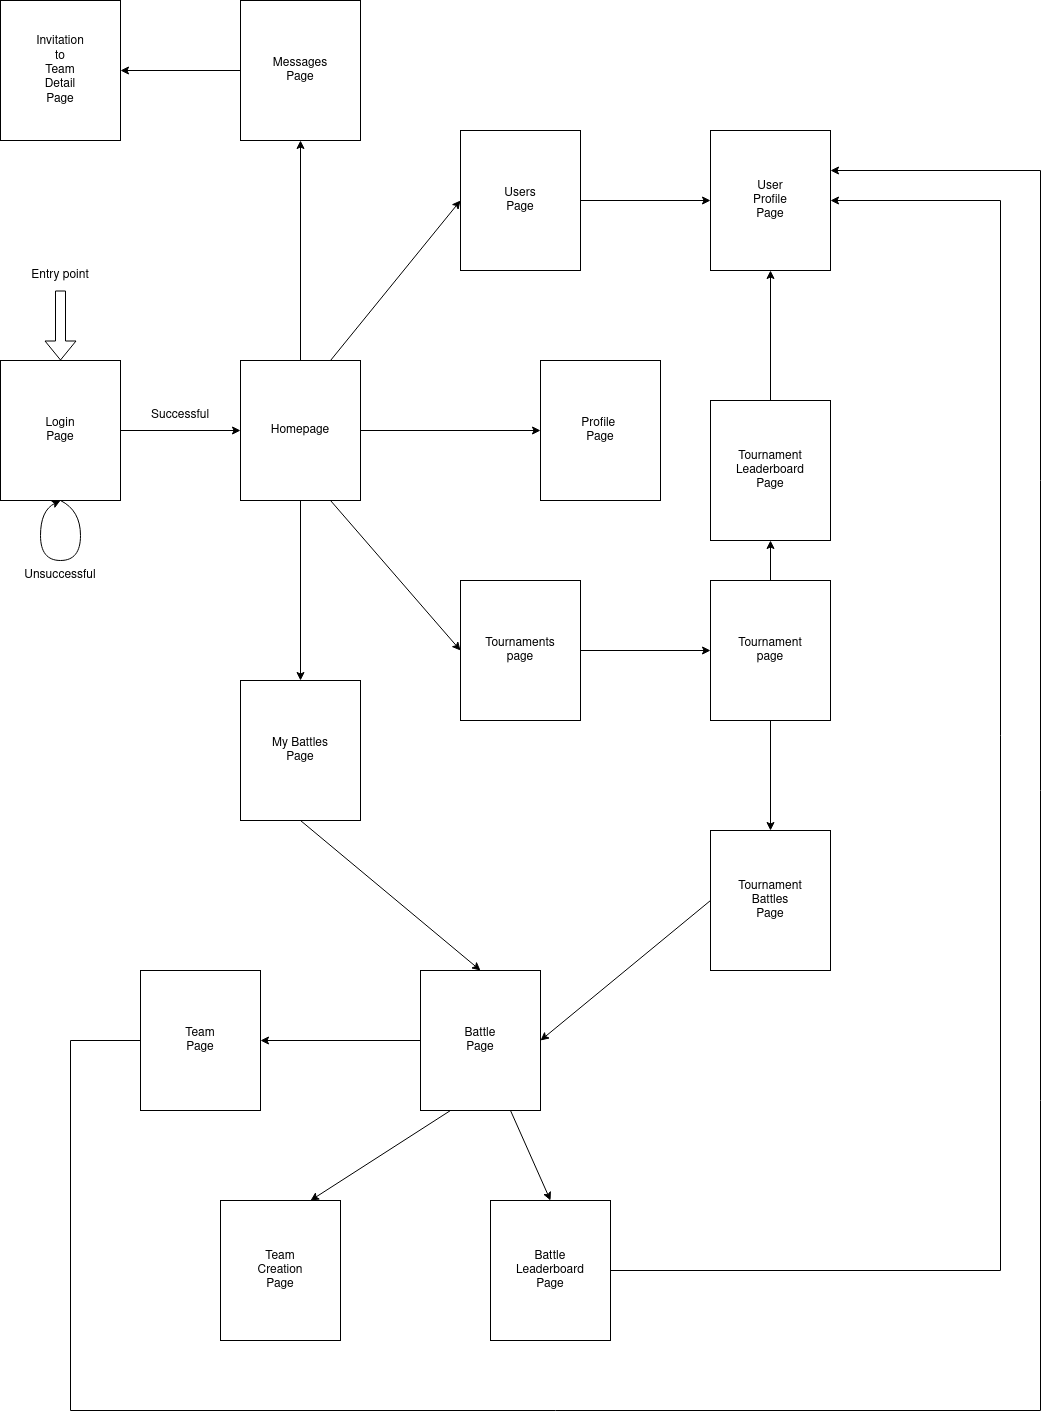
\includegraphics[width=1\linewidth]{Images/designmap.png}
        \caption{Pages of the CKB platform}
        \label{fig: designmap}
    \end{center}
\end{figure}

DESCRIZIONE MAPPA\dots



\section{Registration, Login and Homepage}
\label{sec: registration_login_homepage}%
The following mockups show the SignUp page and the LogIn page. 
Depending on the type of user, the Homepage will be slightly different, as Educators will have a menu entry allowing them to
create new Tournaments or CodeKataBattles directly from the Homepage.

\begin{figure}[H]
    \begin{minipage}{0.45\linewidth}
        \centering
        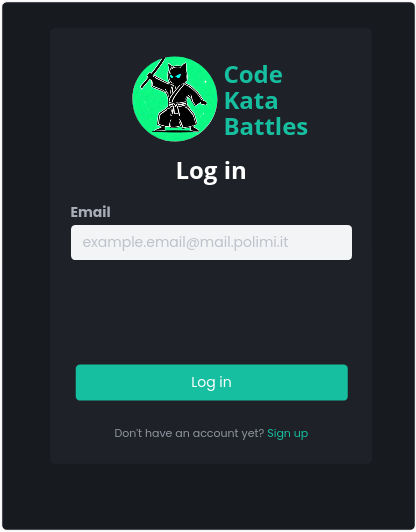
\includegraphics[width=\linewidth]{design/login.png}
        \caption{CKB Log in page}
        \label{fig: login}
    \end{minipage}\hfill
    \begin{minipage}{0.45\linewidth}
        \centering
        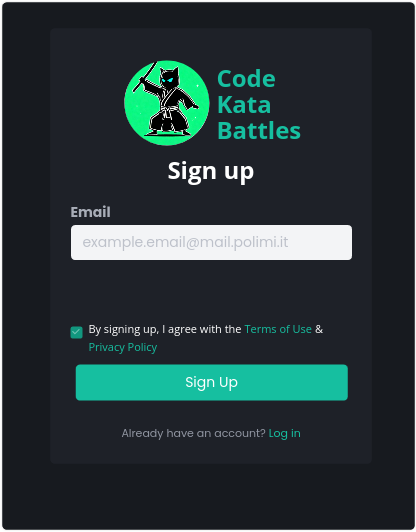
\includegraphics[width=\linewidth]{design/signup.png}
        \caption{CKB Sign Up page}
        \label{fig: signup}
    \end{minipage}
\end{figure}

\begin{figure} [H]
    \begin{center}
        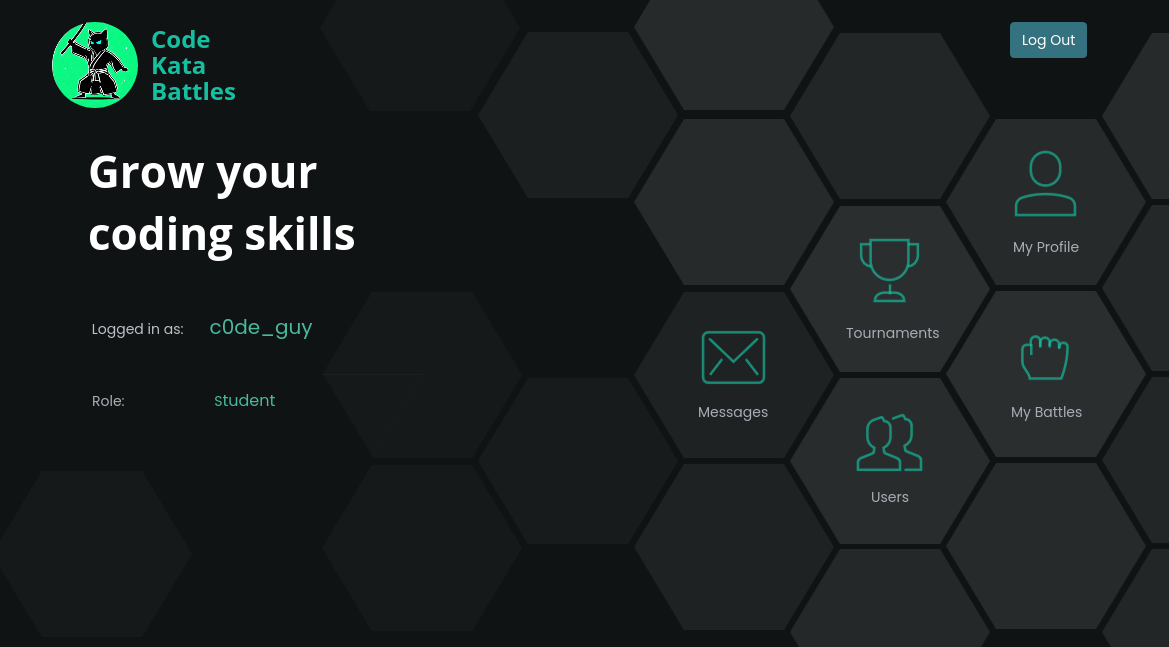
\includegraphics[width=1\linewidth]{design/student_homepage.png}
        \caption{CKB Student Homepage}
        \label{fig: student_homepage}
    \end{center}
\end{figure}

\begin{figure} [H]
    \begin{center}
        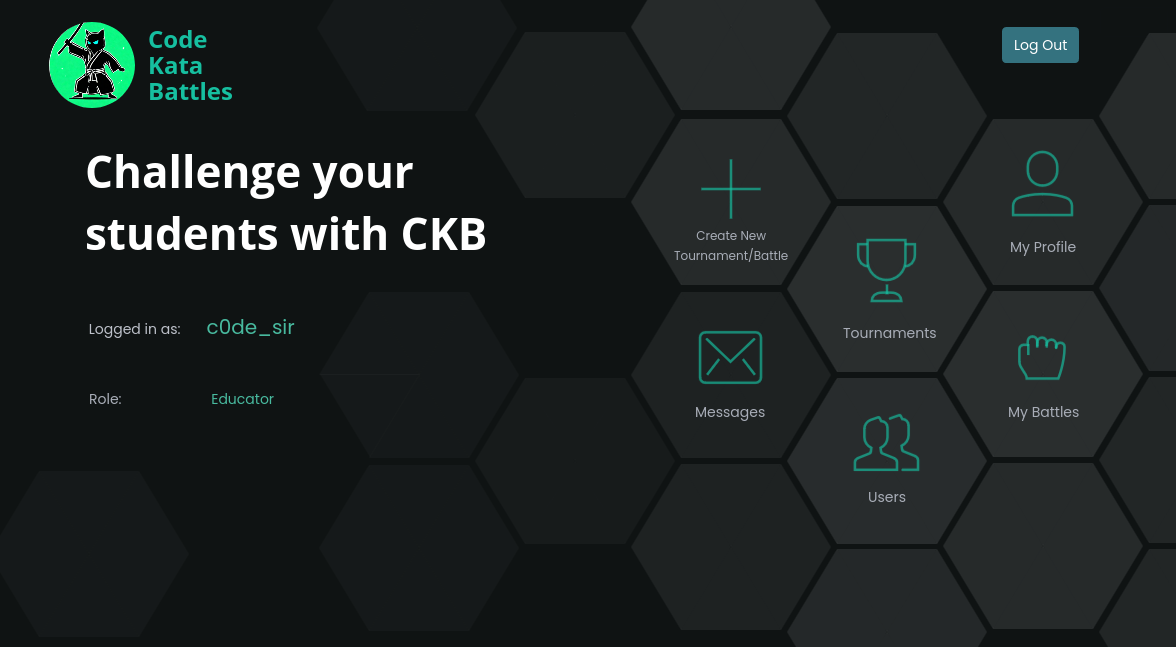
\includegraphics[width=1\linewidth]{design/educator_homepage.png}
        \caption{CKB Educator Homepage}
        \label{fig: educator_homepage}
    \end{center}
\end{figure}

